%capítulo 6
\chapter{Software}

%sección 6.1
\section{Introducción}
Se debe destacar que todo el desarrollo de software se basó exclusivamente en herramientas de software libre. La distribución Linux elegida para el sistema embebido se llama Angström \cite{Angs}. Esta distribución es muy usada en aplicaciones que usan una Beagleboard y cuenta con una gran cantidad de bibliotecas implementadas en lenguaje C, que permiten gran escalabilidad a la hora de incorporar nuevos periféricos en la aplicación.

%sección 6.2
\section{Arquitectura de Software}
%sección 6.2.1
\subsection{Descripción}
Un sistema Linux se compone de diferentes partes que interactúan entre sí, formando capas ordenadas con distintos grados de abstracción respecto al hardware. Ésto lo podemos apreciar en la figura \ref{Fig:SW} donde se muestra a grandes rasgos el sistema implementado. 

\begin{figure}[H]
\centering
  \begin{center}
  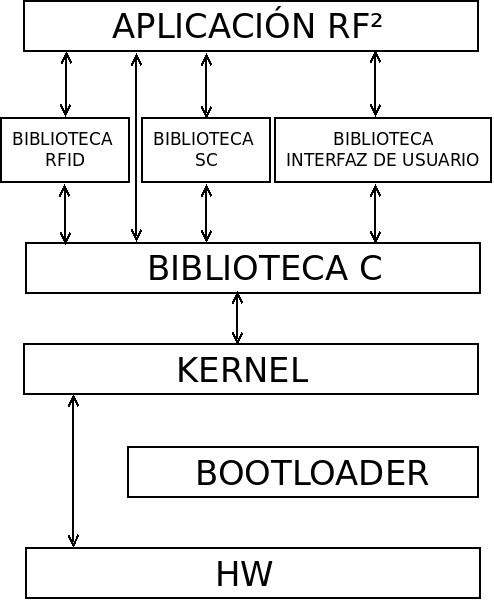
\includegraphics[scale=.4]{Imagenes/SW.jpg} 
  \end{center}
  \caption{Sistema RF${^{2}}$}\label{Fig:SW} 
\end{figure}

El bootloader es la parte del sistema más primitiva y su función es la de cargar el
kernel en memoria RAM para su ejecución. En general el bootloader
es una aplicación que se divide en dos etapas, la primera etapa es fuertemente dependiente
del CPU con que cuenta la placa y su función es buscar en particiones activas para luego cargar 
en memoria RAM la segunda etapa del bootloader. Esta segunda etapa se encarga de descomprimir
en memoria RAM la imagen comprimida del kernel para luego ser ejecutado y que éste tome el
control del sistema.
El kernel se encarga a grandes rasgos de habilitar interrupciones, configurar la memoria y montar un sistema de archivos primitivo que permite a su vez cargar los módulos necesarios para la interfaz con periféricos. Luego se monta el verdadero sistema de archivos (fileSystem). En este nuevo sistema de archivos es donde se instalarán diferentes programas y bibliotecas para la correcta ejecución de aplicaciones.
En funcionamiento, toda la comunicación con periféricos se realiza a través del kernel que es la parte más cercana al hardware.
Cada vez que se ejecuta una aplicación, ésta hace uso de las bibliotecas para poder comunicarse con el kernel, y éste se encarga de la comunicación con los periféricos. Las bibliotecas pueden ser nativas como es el caso de la biblioteca de lenguaje C, o desarrolladas para que determinada aplicación funcione correctamente. 

Una referencia interesante para entender el proceso de arranque es \cite{linuxBoot}.


%sección 6.2.2
\subsection{Sistema Operativo}
En el arranque, la Beagleboard tiene la posibilidad de buscar el bootloader y el kernel en NAND, o en dispositivos extraíbles tales como memorias USB o memorias SD. Para el sistema RF$^{2}$, se eligió un arranque a través de una memoria SD ya que es fácil de manipular.

En la figura \ref{Fig:SD} se puede ver como queda distribuída la memoria SD con las distintas partes
que conforman el sistema operativo. 

\begin{figure}[H]
\centering
  \begin{center}
  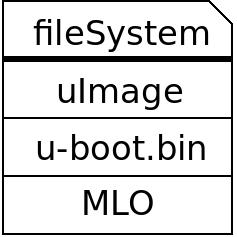
\includegraphics[scale=.4]{Imagenes/sd.jpg} 
  \end{center}
  \caption{Memoria SD para funcionar en Beagleboard}\label{Fig:SD} 
\end{figure}

En la memoria SD se pueden distinguir dos particiones, una en formato FAT32 y otra
en formato ext3. La partición en FAT32 es llamada “de arranque” y es donde se encuentra 
el bootloader (MLO, u-boot.bin) y la imagen comprimida del kernel (uImage). 
La partición en ext3 es donde se encuentra el sistema de archivos (fileSystem).

El MLO es el equivalente al bootloader de la primera etapa, en general ya viene precargado en la memoria NAND de la Beagleboard. Es posible generarlo o incluso bajar una versión ya compilada desde la web de Angström \cite{Angs}. Como característica principal tiene la capacidad de buscar el u-boot.bin en dispositivos extraíbles como memorias SD o USB.

El u-boot.bin es equivalente al bootloader de la segunda etapa. En el sistema RF$^{2}$ fue necesario generarlo ya que tiene la posibilidad de configurar el bloque de expansión de la Beagleboard.

El uImage es el kernel del sistema. Fue necesario generarlo ya que se debieron modificar sus fuentes para que queden habilitadas las interfaces de comunicación con los dispositivos periféricos.

El fileSystem (también conocido como RootFileSystem) es el correspondiente a una distribución Linux llamada Angström. Se pueden llegar a precargar distintos programas y bibliotecas dependiendo de la forma en que se genere.
Angström es una distribución Linux diseñada específicamente para sistemas embebidos desarrollados
para SBCs como la usada para este prototipo. Ésto lo hace más eficiente que otros sistemas operativos para la aplicación desarrollada. La elección de esta distribución se debió a que es de los más recomendados y utilizados en la documentación y foros de Beagleboard \cite{foroBb}.

%sección 6.2.3
\subsection{Bibliotecas}
librfid es una biblioteca open source para manejo de lectores/escritores RFID. Implementa, en el dispositivo lector/escritor, el stack de protocolos ISO 14443A, ISO 14443B, ISO 15693, Mifare Ultralight y Mifare Classic.
Entre los lectores/escritores soportados están OpenPCD y algunos modelos Omnikey, éstos tienen una interfaz de conexión USB. Además, librfib tiene soporte para cualquier otro lector con comunicación directa con el CL RC632 mediante la interfaz SPI y es por esta razón que se tuvo en cuenta.

\bigskip
Existe una herramienta desarrollada que ayuda a entender el funcionamiento de la biblioteca, librfid-tool.

%sección 6.3
\section{Herramientas utilizadas en el desarrollo del sistema}

%sección 6.3.1
\subsection{Introducción}
Para el desarrollo de sistemas existe una gran variedad de herramientas útiles, algunas de software libre y otras privativas. El hecho de tener tantas opciones disponibles, a pesar de ser una ventaja a veces dificulta la elección de las herramientas correctas.

Para la elección de las herramientas se tomó como primer criterio de decisión el hecho que sean libres así como las experiencias de otras personas que ya han transitado caminos comunes, consultando y participando en foros activos.

\bigskip
Cabe señalar que en el PC de desarrollo se utilizó Ubuntu 10.10.

\bigskip
A continuación se detallan las herramientas utilizadas para el desarrollo del sistema. 

%sección 6.3.2
\subsection{MLO, u-boot.bin y uImage}
No fue necesario generar el MLO debido a su simpleza, puesto que el binario precompilado realiza bien su función.

El u-boot.bin y el uImage fueron generados con la herramienta de desarrollo y compilación OpenEmbedded-Bitbake \cite{OE-Bb} que es una fusión de dos herramientas: OpenEmbedded, herramienta para construcción y mantenimiento de distribuciones, y Bitbake, herramienta de compilación similar al Make \cite{Make} que automatiza la construcción de ejecutables entre otros. Esto es, OpenEmbedded utiliza Bitbake para su objetivo. OpenEmbedded-Bitbake es una herramienta muy potente y difícil de aprender al principio. Luego de entendido su principio de funcionamiento se hace muy simple su uso, para lo que es necesario tener acceso a una buena conexión a internet debido a que realiza descargas de paquetes en forma habitual.
Con esta herramienta también se pueden generar el MLO y el fileSystem, aunque se prefirió utilizar otras herramientas por sobre ésta. 
Su instalación, configuración, estructura y uso se pueden ver en el apéndice \ref{anx_sw_oe}.

%sección 6.3.3
\subsection{FileSystem}
Para la generación del fileSystem de Angström, se utilizó la herramienta web Narcissus \cite{Narc} disponible en la página de Angström.
Esta herramienta permite seleccionar entre diferentes dispositivos (entre los cuales está Beagleboard), los programas que se quieran instalar, el formato de la imágen seleccionada, e incluso se puede generar un kit de desarrollo (SDK) para el PC de desarrollo. Debido a la facildad de uso y a los buenos resultados obtenidos, se decidió utilizar esta opción por sobre la del fileSystem generado por la herramienta OpenEmbedded-Bitbake.

%sección 6.3.4
\subsection{Croscompilación}
Se llama croscompilar al proceso de compilación de una arquitectura a otra. En el caso del proyecto RF$^{2}$, se compilan paquetes en una arquitectura x86 (PC de desarrollo) para ser utilizados en una arquitectura ARM.


Para la croscompilación se utilizó el SDK generado por Narcissus y la herramienta Make para generar los archivos necesarios. La instalación, configuración y uso del SDK se encuentran en el apéndice \ref{anx_sw_SDK}.

%sección 6.3.5
\subsection{Depuración de código}
Para la depuración, se utilizó la herramienta GDB del proyecto GNU. 
Al momento de compilar, es necesario agregar la opción -g para que la aplicación pueda ser depurada. Esta opción agrega información en el código de la aplicación.
La interfaz del GDB es por consola, aunque existen algunos programas que utilizan GDB y además ofrecen una interfaz gráfica (DDD \cite{DDD}). \\
Algunos de los comandos útiles y sus usos más comunes pueden encontrarse en el apéndice \ref{depurar}.


\bigskip
Sin olvidar el hecho que la aplicación RF$^{2}$ está diseñada para una arquitectura distinta a la del PC de desarrollo, para el depurado de la aplicación existen dos alternativas. 

La primera opción es lo que se podría llamar depuración local, esto es, instalar GDB en la Beagleboard y depurar la aplicación en ésta. Para saber lo que sucede es necesario acceder de forma remota a la Beagleboard desde el PC de desarrollo. 

La segunda opción es la depuración remota. La depuración remota consiste en realizar la depuración de la aplicación desde el PC de desarrollo. Para esto, es necesario instalar GDBServer en la Beagleboard y tener instalado el GDB específico de la Beagleboard en el PC de desarrollo. Luego se establece una conexión, serial o ethernet, entre la Beagleboard y el PC de desarrollo. Por más detalles sobre la configuración referirse al apéndice \ref{GDB}.

\bigskip
La primera opción no es posible para sistemas embebidos chicos en los cuales no se puede instalar GDB, aunque éste no es el caso de la Beagleboard. 
Se tienen más y mejores herramientas en el PC de desarrollo, por ejemplo programas con interfaz gráfica que ayudan a entender mejor lo que está pasando. Por algunas de estas razones, se prefiere el uso de la depuración remota. 

\bigskip
Se utilizaron indistintamente tanto la primera opción como la segunda.

%sección 6.3.6
\subsection{Bibliotecas}

\begin{itemize}
\item pcsc-scan es una herramienta de uso por línea de comandos, que una vez ejecutado imprime el nombre del lector PC/SC conectado y en caso que exista una tarjeta de contacto insertada imprime también su ATR. Luego  escanea el lector constantemente e indica si se retira o inserta una tarjeta.
\item  librfid-tool es una herramienta de uso por línea de comandos que da acceso de bajo nivel RFID utilizando los lectores soportados por la librfid.
\end{itemize}

A continuación se detallan la forma de llamar a la aplicación y algunas de las opciones soportadas. Para la instalación y uso referirse al apéndice \ref{ins_conf_librfid}

%sección 6.3.7
\subsection{Otras herramientas}
subversion y Git, para control de versiones. 

Geany para edición y compilación de código.

minicom para comunicación serial.

strace es un comando linux que lista las llamadas al sistema, útil para la depuración.

%sección 6.4
\section{Desarrollo}

%sección 6.4.1
\subsection{MLO}
Como se mencionó anteriormente, no fue necesario generar el MLO debido a que la Beagleboard viene con uno pre-instalado, y en caso de que no funcione en forma correcta se puede descargar desde un repositorio de Angström \cite{Angs_MLO}. No fue necesario realizar ningún cambio en el archivo ya que realiza su función correctamente.

%sección 6.4.2
\subsection{Multiplexado de pines}
El microprocesador OMAP3530 tiene muchos pines con distintas interfaces entre las
que se cuentan puertos UART, SPI, GPIO, etc., pero no todos son accecibles desde la Beagleboard. 
Para poder acceder a algunos de estos puertos del microprocesador, existe en la placa de la
Beagleboard un bloque de expansión de 28 pines.

\bigskip
Por defecto, en el bloque de expansión no se encuentran las señales que se quieren. Esto 
lleva a que se tenga que modificar el estado inicial de los pines. 
Existen dos formas de modificar los pines de modo de tener las señales que se precisan. Una de ellas es modificar el bootloader y la otra es modificar el kernel. Esto implica cambios en los archivos fuentes y posterior compilación que genere los nuevos binarios u-boot o uImage. 

\bigskip
Para la modificación de las señales disponibles en el bloque de expansión se decidió modificar el u-boot ya que la modificación por u-boot es más intuitiva y por experiencia se sabe que lo que más se actualiza y/o modifica es el kernel. 

%sección 6.4.3
\subsection{u-boot}
Como se mencionó anteriormente en el u-boot se realizó la configuración de los pines del bloque de expansión de la Beagleboard. 
Cada pin del bloque de expansión tiene varias funcionalidades asociadas, y la configuración de la 
funcionalidad depende de un multiplexado modificable a nivel de software. Esto es, dependiendo del “modo de pin” elegido, la función que se obtiene en dicho pin.
Para que los cambios hechos en el u-boot tengan el efecto esperado al arrancar el sistema, es necesario que en la configuración del kernel esté la opción CONFIG\_OMAP\_MUX=no, lo que imposibilita al kernel a realizar este mismo cambio. Esta opción no está activada por defecto para versiones de kernel 2.6.32 y posteriores. 

\bigskip
Antes que pueda ser modificado el estado de los pines del bloque de expansión,
es necesario obtener los archivos fuente con los cuales se genera el archivo binario u-boot.

\bigskip
Nota: Puede que cuando se realiza la instalación de OpenEmbedded-Bitbake, se genere un directorio relacionado con u-boot en /stuff/build/tmp/work/beagleboard-angstrom-linux-gnueabi/, si esto es así, no es necesario volver a obtener los fuentes.

\bigskip
\leftline{Se configura el bitbake para poder utilizarlo:}

\bigskip
\centerline{\$ export BBPATH=/stuff/build:/stuff/openembedded}

\centerline{\$ export PATH=/stuff/bitbake/bin:\$PATH}

\bigskip
\leftline{Se obtienen los fuentes:}

\centerline{\$ cd /stuff/build}

\centerline{\$ bitbake -f -c clean -b ../openembedded/recipes/u-boot/u-boot\_git.bb}

\centerline{\$ bitbake -f -c compile -b ../openembedded/recipes/u-boot/u-boot\_git.bb}

\bigskip
Los fuentes se encuentran en 

/stuff/build/tmp/work/beagleboard-angstrom-linux-gnueabi/u-boot.../git/.

\bigskip
En los fuentes del u-boot dentro de board/ti/beagle/ se encuentra el archivo beagle.h que es donde se establece la configuración de los pines del bloque de expansión de la Beagleboard.

Si se abre este archivo se ven líneas del estilo: 

\begin{verbatim}
MUX_VAL(CP(MCBSP3_DX), (IEN | PTD | DIS | M4)) /*GPIO_140*/\
\end{verbatim}

MUX\_VAL indica que se va a modificar el valor de multiplexado de lo que está entre paréntesis. 

\bigskip
CP(MCBSP3\_DX) es el Control\_PadConf, esto es el registro del microprocesador asociado con el 
pin a modificar. 

\bigskip
(IEN $|$ PTD $|$ DIS $|$ M4) esta es la configuración del pin en cuestión: 


La opción IEN (input enable) hace que el pin sea bidireccional. 

La opción PTD y PTU, indica si el pin tiene un pull down o pull up respectivamente. 

La opción DIS y EN, indica si se deshabilitan o no las opciones PTD y PTU respectivamente. 

La opción M4 es el modo seleccionado para el pin. Para la Beagleboard existen cuatro modos: M1, M2, M3 y M4.

\bigskip
GPIO\_140 es el nombre del pin (solo es un comentario). 

\bigskip
El Control\_PadConf es un registro de 32bits el cual controla el estado de dos pines, esto es, la parte 
baja del registro controla un pin y la parte alta controla otro. 

Analizando el “manual de referencia Beagleboard del usuario” (“Expansion connector signals” – tabla 20), y “manual técnico de referencia OMAP35x” (“SCM functional description” – capítulo 7.4.4); ambos adjuntos en el apéndice \ref{HD}; y agregando las opciones que interesan para los pines, se confeccionó la siguiente tabla: 

\begin{longtable}{|c|p{2.6cm}|c|p{2.5cm}|c|}
\hline
\textbf{CONTROL\_PADCONF\_} & \textbf{EQUIV. BEAGLE.H} & \textbf{PIN EXPANSIÓN} & \textbf{SEÑAL EN EL PIN} & \textbf{MODO} \\ \hline
MMC2\_DAT6[31:16] & MMC2\_DAT7 & 3 & GPIO\_139 & 4 \\ \hline
UART2\_CTS[15:0] & UART2\_CTS & 4 & GPIO\_144 & 4 \\ \hline
MMC2\_DAT6[15:0] & MMC2\_DAT6 & 5 & GPIO\_138 & 4 \\ \hline
UART2\_TX[15:0] & UART2\_TX & 6 & UART2\_TX & 0 \\ \hline
MMC2\_DAT4[31:16] & MMC2\_DAT5 & 7 & GPIO\_137 & 4 \\ \hline
McBSP3\_CLKX[31:16] & McBSP3\_FSX & 8 & UART2\_RX & 1 \\ \hline
MMC2\_DAT4[15:0] & MMC2\_DAT4 & 9 & GPIO\_136 & 4 \\ \hline
UART2\_CTS[31:16] & UART2\_RTS & 10 & GPIO\_145 & 4 \\ \hline
MMC2\_DAT2[31:16] & MMC2\_DAT3 & 11 & McSPI3\_CS0 & 1 \\ \hline
McBSP1\_DX[15:0] & McBSP1\_DX & 12 & GPIO\_158 & 4 \\ \hline
MMC2\_DAT2[15:0] & MMC2\_DAT2 & 13 & GPIO\_134 & 4 \\ \hline
McBSP1\_CLKX[15:0] & McBSP1\_CLKX & 14 & GPIO\_162 & 4 \\ \hline
MMC2\_DAT0[31:16] & MMC2\_DAT1 & 15 & GPIO\_133 & 4 \\ \hline
McBSP\_CLKS[31:16] & McBSP1\_FSX & 16 & GPIO\_161 & 4 \\ \hline
MMC2\_DAT0[15:0] & MMC2\_DAT0 & 17 & McSPI3\_SOMI & 1 \\ \hline
McBSP1\_DX[31:16] & McBSP1\_DR & 18 & GPIO\_159 & 4 \\ \hline
MMC2\_CLK[31:16] & MMC2\_CMD & 19 & McSPI3\_SIMO & 1 \\ \hline
McBSP1\_CLKR[15:0] & McBSP1\_CLKR & 20 & GPIO\_156 & 4 \\ \hline
MMC2\_CLK[15:0] & MMC2\_CLK & 21 & McSPI3\_CLK & 1 \\ \hline
McBSP1\_CLKR[31:16] & McBSP1\_FSR & 22 & GPIO\_157 & 4 \\ \hline
I2C2\_SDA[15:0] & I2C2\_SDA & 23 & GPIO\_183 & 4 \\ \hline
I2C1\_SDA[31:16] & I2C2\_SCL & 24 & GPIO\_168 & 4 \\ \hline
\caption{Modo de pines en bloque de expansión}\label{pines}
\end{longtable}


Al modificar el archivo beagle.h hay que tener mucho cuidado ya que al sustituir los valores no se deben repetir pines ni registros, no deben haber incoherencias, un registro por cada pin y un pin por cada registro. 
Dentro del archivo hay un macro definido MUX\_BEAGLE\_C(), donde se deben realizar las modificaciones ya que este macro está asociado con el modelo de Beagleboard utilizado (C4).\\
En una primera instancia se sustituyeron los valores del cuadro \ref{pines} buscando los equivalentes del 
PadConf en el archivo beagle.h. 


\begin{verbatim}
\#define MUX_BEAGLE_C() \
MUX_VAL(CP(MCBSP3_DX),   (IEN  | PTD | DIS | M4))/*GPIO_140*/\
MUX_VAL(CP(MCBSP3_DR),   (IEN  | PTD | DIS | M4))/*GPIO_142*/\
MUX_VAL(CP(MCBSP3_CLKX), (IEN  | PTD | DIS | M4))/*GPIO_141*/\
MUX_VAL(CP(MCBSP3_FSX),  (IEN  | PTD | DIS | M1))/*UART2_RX*/\
MUX_VAL(CP(UART2_TX),    (IDIS | PTD | DIS | M0))/*UART2_TX*/\
MUX_VAL(CP(MMC2_DAT7),   (IEN  | PTD | EN  | M4))/*GPIO_139*/\
MUX_VAL(CP(UART2_CTS),   (IEN  | PTD | DIS | M4))/*GPIO_144*/\
MUX_VAL(CP(MMC2_DAT6),   (IEN  | PTD | EN  | M4))/*GPIO_138*/\
MUX_VAL(CP(MMC2_DAT5),   (IEN  | PTD | EN  | M4))/*GPIO_137*/\
MUX_VAL(CP(MMC2_DAT4),   (IEN  | PTD | EN  | M4))/*GPIO_136*/\
MUX_VAL(CP(UART2_RTS),   (IEN  | PTD | EN  | M4))/*GPIO_145*/\
MUX_VAL(CP(MCBSP1_DX),   (IEN  | PTD | EN  | M4))/*GPIO_158*/\
MUX_VAL(CP(MMC2_DAT2),   (IEN  | PTD | EN  | M4))/*GPIO_134*/\
MUX_VAL(CP(MCBSP1_CLKX), (IEN  | PTD | EN  | M4))/*GPIO_162*/\
MUX_VAL(CP(MMC2_DAT1),   (IEN  | PTU | EN  | M4))/*GPIO_133*/\
MUX_VAL(CP(MCBSP1_FSX),  (IEN  | PTD | EN  | M4))/*GPIO_161*/\
MUX_VAL(CP(MCBSP1_DR),   (IEN  | PTD | EN  | M4))/*GPIO_159*/\
MUX_VAL(CP(MCBSP1_CLKR), (IEN  | PTD | EN  | M4))/*GPIO_156*/\
MUX_VAL(CP(MCBSP1_FSR),  (IEN  | PTD | EN  | M4))/*GPIO_157*/\
MUX_VAL(CP(I2C2_SDA),    (IEN  | PTD | EN  | M4))/*GPIO_183*/\
MUX_VAL(CP(I2C2_SCL),    (IEN  | PTU | EN  | M4))/*GPIO_168*/\
MUX_VAL(CP(MMC2_DAT3),   (IEN  | PTD | EN  | M1))/*SPI3_CS0*/\
MUX_VAL(CP(MMC2_DAT0),   (IEN  | PTU | EN  | M1))/*SPI3_SOMI*/\
MUX_VAL(CP(MMC2_CMD),    (IEN  | PTU | DIS | M1))/*SPI3_SIMO*/\
MUX_VAL(CP(MMC2_CLK),    (IEN  | PTU | DIS | M1))/*SPI3_CLK*/
\end{verbatim}

Luego es necesario compilar para obtener el u-boot.bin.

\bigskip
\centerline{\$ cd /stuff/build}

\centerline{\$ bitbake -f -c compile -b ../openembedded/recipes/u-boot/u-boot\_git.bb}

\centerline{\$ bitbake -f -c deploy -b ../openembedded/recipes/u-boot/u-boot\_git.bb}

\bigskip
Nota: Cada vez que se introduzca un nuevo cambio, no es necesario ejecutar el comando con la opción clean (lo que implica volver a bajar los fuentes), solo basta con volver a compilar.

\bigskip
El archivo generado (u-boot.bin) se encuentra en 

/stuff/build/tmp/deploy/glibc/images/beagleboard/ aunque con su nombre seguido de un número identificatorio, el cual debe ser borrado para poder mantener el nombre necesario (u-boot.bin).

\bigskip
Pese a que en la literatura y foros, se plantea lo contrario, no fue posible establecer los atributos “valor” y “dirección” de los pines GPIO mediante la modificación planteada (una posible solución puede verse en el apéndice \ref{anx_sw_uIm}). Lo que sí cambia efectivamente es el modo del pin, permitiendo obtener las interfaces adecuadas en el bloque de expansión.

%sección 6.4.4
\subsection{uImage}
La versión del kernel elegida fue la 2.6.32 ya que en el momento del desarrollo era la versión más estable. Aunque también se hicieron pruebas con las versiones 2.6.29 y 2.6.37.\\
Durante el arranque del sistema, el kernel carga los módulos y controladores necesarios para el funcionamiento del 
hardware que forma parte del sistema embebido. También se montan las interfaces para poder interactuar con los distintos dispositivos a ser conectados a la Beagleboard como lo son: SPI, GPIO, UART, etc. Las interfaces SPI y UART se encuentran bajo el directorio /dev en el sistema de archivos, y GPIO bajo el directorio /sys/class/gpio. En algunos casos, en /dev no aparecen algunas de las interfaces configuradas, lo que lleva a modificar los fuentes del kernel para que esto así suceda. Este fue el caso de la interfaz SPI que no quedó mapeada en /dev pese a que había sido configurada en los fuentes del u-boot. También hubo problemas con los atributos “valor” y “dirección” de los GPIO, como se mencionó anteriormente. Adicionalmente hacía falta un módulo para simular una conexión ethernet sobre una interfaz USB para establecer una conexión entre la Beagleboard y un PC como si fuera un enlace de red. 
Todo esto llevó a que se tuvieran que modificar los archivos fuente del kernel.

\bigskip
A continuación se detallan los pasos a seguir para la modificación de los fuentes del kernel:
 
\bigskip 
Comando necesario para el desarrollo del uImage:

\bigskip
\centerline{\$ bitbake virtual/kernel -c [comando]}

\bigskip
virtual/kernel: refiere a que se quiere generar un kernel.

\bigskip
Entre los comandos:

\bigskip
clean: borra el contenido del directorio work. Borra todos los cambios hechos en la configuración del uImage fuente y parches agregados.

patch: genera los archivos de configuración y el fuente del uImage. Además le aplica los parches.

menuconfig: abre el editor de la configuración del kernel.

compile: compila todo.

deploy: genera los archivos referidos en este caso al uImage (.config, módulos, uImage) y los guarda en el directorio /stuff/build/tmp/deploy/glibc/images/beagleboard/.

\bigskip
Nota: Es necesario que todos estos comandos sean ejecutados en el orden adecuado para que todo funcione correctamente.

\bigskip
Primero se configura bitbake para poder utilizarlo:

\centerline{\$ export BBPATH=/stuff/build:/stuff/openembedded}

\centerline{\$ export PATH=/stuff/bitbake/bin:\$PATH}

\bigskip
Se comienza el desarrollo:

\centerline{\$ cd /stuff/build}

\centerline{\$ bitbake virtual/kernel -c clean}

\centerline{\$ bitbake virtual/kernel -c patch}

\centerline{\$ bitbake virtual/kernel -c menuconfig}

\bigskip
Luego de ejecutar este comando se abre el editor de la configuración del kernel (ver figura \ref{Fig:kernel}). Este editor indica qué módulos cargar y cuáles no. En este caso un cambio de  configuración es necesario para el buen funcionamiento de la interfaz SPI y de la conexión USB-ethernet con la Beagleboard.

\begin{figure}[H]
\centering
  \begin{center}
  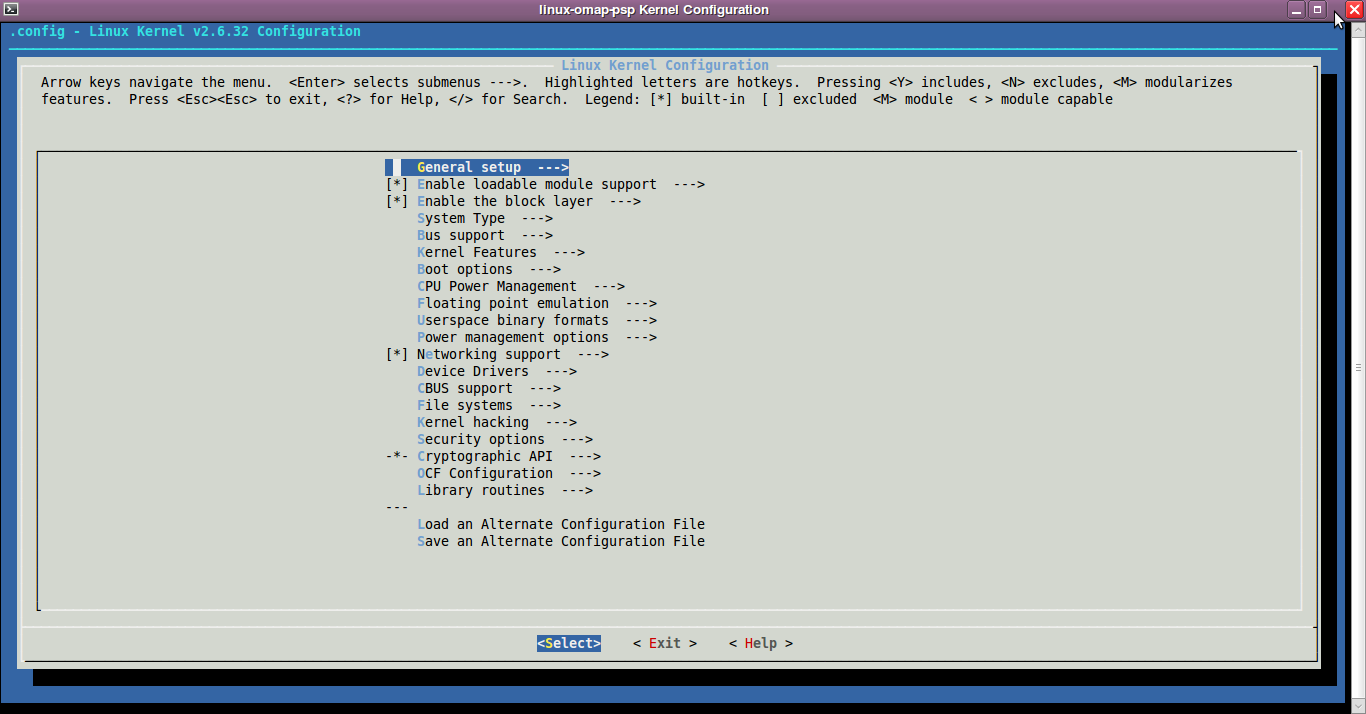
\includegraphics[scale=.3]{Imagenes/kernel.png} 
  \end{center}
  \caption{Editor de configuración del kernel}\label{Fig:kernel} 
\end{figure}

Para configurar la interfaz SPI, se debe configurar como sigue:

Device Drivers – SPI Support=y y luego como en la figura \ref{Fig:spi}.

\begin{figure}[H]
\centering
  \begin{center}
  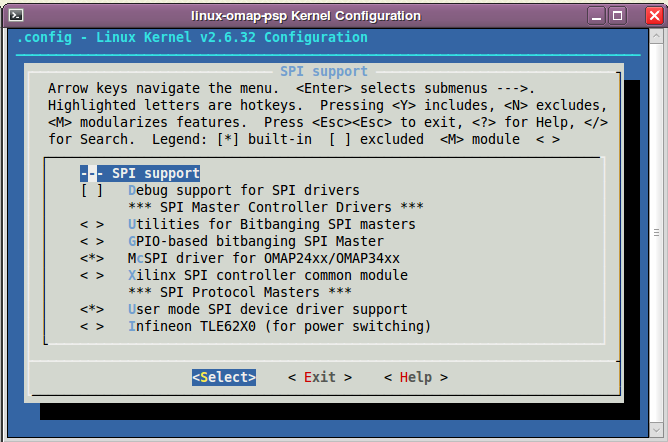
\includegraphics[scale=.4]{Imagenes/spi_chica.png} 
  \end{center}
  \caption{Configuración SPI}\label{Fig:spi} 
\end{figure}


Para poder establecer la conexión por USB con la Beagleboard, se debe configurar como sigue: 

Device Drivers – USB Support=y – USB Gadget Support=y y luego como en la figura \ref{Fig:usb}.

\begin{figure}[H]
\centering
  \begin{center}
  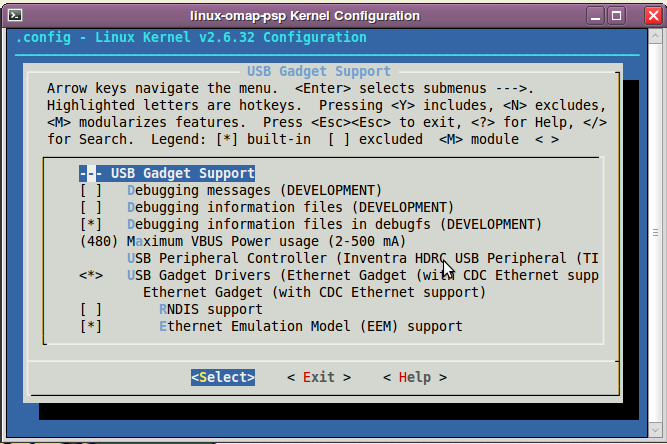
\includegraphics[scale=.4]{Imagenes/usb_chica.png} 
  \end{center}
  \caption{Configuración USB Gadget}\label{Fig:usb} 
\end{figure}

Luego, es necesario modificar el archivo board\_omap3beagle.c que se encuentra en /stuff/build/tmp/work/beagleboard-angstrom-linux-gnueabi/linux-omap-.../git/arch/arm/mach-omap2/. En este archivo está toda la inicialización de las interfaces. Los detalles de los cambios introducidos en este archivo se pueden observar en el apéndice \ref{anx_sw_uIm}.

\bigskip
Se compila y genera el archivo uImage:

\bigskip
\centerline{\$ bitbake virtual/kernel -c compile}

\centerline{\$ bitbake virtual/kernel -c deploy}

\bigskip
Dentro de /stuff/build/tmp/deploy/glibc/images/beagleboard/ se encuentra el archivo uImage generado.

\bigskip
Nota: Respecto al nombre del archivo, al igual que con el caso del u-boot.bin el nombre que aparece es un nombre más largo y necesita ser renombrado a uImage para que se pueda ejecutar correctamente.

%sección 6.4.5
\subsection{FileSystem}

Como se mencionó anteriormente, el fileSystem se generó a partir de la herramienta web Narcissus.\\
En el fileSystem es donde se encuentran los paquetes y programas ya instalados. Cuanto más programas se instalen más grande será en tamaño el fileSystem.

\bigskip
Para utilizar la herramienta Narcissus se debe acceder a la web de la herramienta \cite{Narc}.

\bigskip
A continuación se detallan las diferentes características y opciones que se eligieron para crear un fileSystem a medida para la Beagleboard y un SDK para el PC de desarrollo:

\bigskip
Select Machine: Beagleboard.

\bigskip
Image Name: el nombre que se le quiera dar.

\bigskip
Complexity: complejidad, se eligió “advanced” ya que la opción “simple” no brinda libertad de configuración.

\bigskip
Release: versión, aquí hay varias opciones disponibles, se eligió “unstable” ya que es la más estable de las disponibles. La primera opción disponible es la más estable.

\bigskip
Base System: aquí se elige el soporte de drivers y paquetes que se pretenden. “bare bones” es la opción con menos soporte y “extended” es la de mayor soporte. Cuanto más soporte, más pesado se hace el fileSystem. Una opción interesante es la opción “regular”, y es la que se eligió.

\bigskip
/dev manager: esto es el manejador de /dev, se recomienda “udev”.

\bigskip
Type of Image: formato en el que se quiere descargar el fileSystem. Se eligió “tar.gz” ya que es la opción más versátil.

\bigskip
Software manifest: se genera un archivo en la web con todos los paquetes que se instalaron en detalle.

\bigskip
SDK type: esta opción permite generar un SDK para el PC de desarrollo compatible con el fileSystem generado. Esto es sumamente útil por ejemplo para croscompilar. Aquí se eligió la opción “Full SDK”.

\bigskip
User environment section: aquí se indica que tipo de sistema operativo se quiere, básicamente se tienen dos opciones; una es un fileSystem sin interfaz gráfica y las otra con entorno gráfico. Se eligió la opción “console” (sin entorno gráfico) ya que la aplicación no exige entorno gráfico.

\bigskip
Luego se permite seleccionar programas que se desean instalar.
Las aplicaciones elegidas son: nano editor (editor de texto) ya que hace las cosas más fáciles que el programa vi, GDB y GDBServer necesarios para la depuración de la aplicación, y toolchain para tener herramientas de compilación nativas en la Beagleboard.

\bigskip
Cuando todo fue seleccionado, se da un click en “build me” (demora un poco).
Cuando el proceso termina, se generan dos archivos comprimidos, un archivo con el nombre elegido para la imagen en un formato .tar.gz y el SDK para el PC de desarrollo en formato .tar.bz2. 

%sección 6.4.6
\subsection{Beagleboard}

\subsubsection{Preparación de la memoria SD}

Con los archivos MLO, u-boot.bin, uImage y fileSystem generados, se procede a la preparación de la memoria SD para correr por primera vez en la Beagleboard. En el apéndice \ref{sd_prep} se describen los pasos necesarios para el correcto funcionamiento del sistema.


\subsubsection{Configuración de los parámetros de arranque}

Existe una forma de saber lo que sucede en el arranque del sistema conectando la Beagleboard a un PC a través de un cable con conversor USB-SERIAL y utilizando la interfaz serial de la Beagleboard (/dev/ttyS2) para la comunicación con el PC.

\bigskip
Para saber sobre la configuración en el PC para conexión serial con la Beagleboard ver apéndice \ref{serialBb}.

\leftline{Primer arranque de la Beagleboard}

\bigskip
Para evitar problemas, se recomienda alimentar la Beagleboard con el transformador correspondiente.

\bigskip
Antes de arrancar se abre minicom por consola: 

\bigskip
\centerline{\$ minicom}

\bigskip
Se coloca la SD en la Beagleboard, se enchufa, y comienza el arranque del sistema. 

Para que el sistema arranque correctamente con los archivos generados previamente, se debe mantener presionado el botón “user” de la Beagleboard ya que en caso contrario en el arranque se busca el u-boot.bin primero en NAND y si ya existe una versión preinstalada es ésta la que se va a cargar. Al apretar el botón “user” (no más de tres segundos) se logra un cambio en el orden de arranque lo que hace que se cargue primero el u-boot.bin de la memoria SD.

Luego se debe ver una cuenta regresiva en pantalla. 
Si se apreta alguna tecla del teclado esta cuenta regresiva se detiene y se accede a la configuración de los parámetros de arranque del sistema (similar a una BIOS de un PC de escritorio). Para ver una lista de todas los parámetros del arranque, se debe ejecutar el comando printenv. En el apéndice \ref{printenv} puede verse el listado que devuelve la ejecución de dicho comando.

\bigskip
Entre los parámetros a modificar están los que indican como acceder a la SD (bootargs) y los comandos de arranque (bootcmd) donde se indica en que lugar encontrar el uImage. Para un arranque correcto a través de la SD, los valores de los parámetros anteriores deben ser los siguientes:

\begin{verbatim}
bootargs= 'console=ttyS2,115200n8 root=/dev/mmcblk0p2 
rw rootwait' 
bootcmd 'mmc init;fatload mmc 0 80300000 uImage;
bootm 80300000' 
\end{verbatim}

En general esto ya viene seteado correctamente. Si no es así, van a haber errores al arrancar el sistema. Una solución es setear los valores de estos atributos mediante el comando setenv:

\begin{verbatim}
OMAP3 beagleboard.org # setenv bootargs 'console=ttyS2,115200n8 
root=/dev/mmcblk0p2 rw rootwait' 

OMAP3 beagleboard.org # setenv bootcmd 'mmc init;fatload mmc 
0 80300000 uImage;bootm 80300000' 

OMAP3 beagleboard.org # saveenv 
\end{verbatim}

Nota: saveenv guarda los valores seteados en NAND.

\bigskip
También se puede modificar el tiempo de la cuenta regresiva (bootdelay) mencionada anteriormente para lograr un mejor tiempo de arranque.

\begin{verbatim}
OMAP3 beagleboard.org # setenv bootdelay 1

OMAP3 beagleboard.org # saveenv 
\end{verbatim}

Luego de aplicados los cambios en los parámetros de arranque, se reinicia el sistema.

\begin{verbatim}
OMAP3 beagleboard.org # reset 
\end{verbatim}

Un ejemplo de arranque del sistema puede verse en el apéndice \ref{arr}.

\subsubsection{Copia de MLO y u-boot.bin en NAND}

Recordando que se debe dejar apretado el botón “user” de la Beagleboard para lograr que se cargue el u-boot.bin de la memoria SD y no el de la NAND (por defecto), y dado que esto no es conveniente para un sistema que pretende ser autónomo, se decidió copiar los archivos MLO y u-boot.bin a la memoria NAND. Esta operación es muy delicada y se deben seguir los pasos que se mencionan a continuación al pie de la letra, ya que cualquier error puede dejar inservible a la Beagleboard. Antes de hacer esto es conveniente tener la versión definitiva de los archivos a copiar ya que la NAND es una memoria delicada.

\bigskip
Se accede a la ventana de cambios en los parámetros de arranque y se realiza lo siguiente:

\begin{verbatim}
OMAP3 beagleboard.org # mmc init 
mmc1 is available 
OMAP3 beagleboard.org # fatload mmc 0:1 80000000 MLO 
reading MLO 
19908 bytes read 
\end{verbatim}

Primero se inicializa el subsistema mmc para la memoria SD y luego se copia de la partición 1 de la mmc 0 el archivo MLO en la dirección 80000000.

\bigskip
Para escribir en la NAND se debe habilitar la siguiente funcionalidad.
\begin{verbatim}
OMAP3 beagleboard.org # nandecc hw 
HW ECC selected 
\end{verbatim}

Se borran las direcciones de memoria en donde se quiere escribir.
\begin{verbatim}
OMAP3 beagleboard.org # nand erase 0 80000 
NAND erase: device 0 offset 0x0, size 0x80000 
Erasing at 0x60000 -- 100% complete. 
OK 
\end{verbatim}

Se copia en NAND el MLO.

\begin{verbatim}
OMAP3 beagleboard.org # nand write 80000000 0 80000 
NAND write: device 0 offset 0x0, size 0x80000 
524288 bytes written: OK 
\end{verbatim}

Para copiar el u-boot se procede d ela misma manera.

\begin{verbatim}
OMAP3 beagleboard.org # mmc init 
mmc1 is available 
OMAP3 beagleboard.org # fatload mmc 0:1 80000000 u-boot.bin 
reading u-boot.bin 
188600 bytes read 
OMAP3 beagleboard.org # nandecc sw 
SW ECC selected 
OMAP3 beagleboard.org # nand erase 80000 160000 
NAND erase: device 0 offset 0x80000, size 0x160000 
Erasing at 0x1c0000 -- 100% complete. 
OK 
OMAP3 beagleboard.org # nand write 80000000 80000 160000 
NAND write: device 0 offset 0x80000, size 0x160000 
1441792 bytes written: OK
\end{verbatim}

\subsubsection{Beagleboard en la red}

Es de interés conectar la Beagleboard a través de una interfaz ethernet con el PC de desarrollo para poder intercambiar archivos e incluso conectar la Beagleboard a internet. Para lograr lo anterior se agregaron los módulos necesarios durante el desarrollo del uImage. Para la emulación de la conexión por red se utiliza el USB-OTG de la Beagleboard.

\bigskip
\leftline{Conexión con beagle a través del USB-OTG}

\bigskip
Tener una conexión por red con la BeagleBoard permite el uso de comandos como ssh para acceso remoto y el envío de archivos mediante el comando scp. 
Si se conecta la Beagleboard con el PC de desarrollo, se puede ver en el PC la aparición de una conexión de red mediante la interfaz usb0. Se debe configurar esta interfaz como sigue:

\bigskip
\centerline{\$ ifconfig usb0 172.16.1.17 netmask 255.255.255.0}

\bigskip
La única condición que debe tener la ip es que no sea parte de la subred a la que pertenece el PC desarrollo (en general 192.168.x.x) ya que esto lleva a errores de comunicación y por ejemplo, no permite la salida de la Beagleboard a internet.

\bigskip
Para que se establezca la conexión es necesaria la ejecución de algunos comandos en la Beagleboard, por ejemplo interesa una ip fija para identificarla en la red. Para que la conexión se realice cada vez que se inicia el sistema, se creó un script (ethusb) que se corre al inicio y ejecuta los comandos antes mencionados.
A continuación se muestra el script ethusb:

\begin{verbatim}
#!/bin/sh 
echo Ya se puede conectar... 
ifconfig usb0 172.16.1.14 netmask 255.255.255.0 
route add default gw 172.16.1.17 
echo nameserver 192.168.1.2 > /etc/resolv.conf 
\end{verbatim}

Se configura la ip que va a tener la Beagleboard. La puerta de enlace debe ser la ip del PC de desarrollo y el nameserver debe ser la dirección de la ip de salida a internet que tiene la PC de desarrollo.

\bigskip
Para que el script se ejecute cada vez que arranca el sistema, se debe hacer lo siguiente:

\bigskip
\centerline{\$ cp ethusb /etc/init.d}

\centerline{\$ cd /etc/rc5.d}

\centerline{\$ ln -s ../init.d/ethusb S99ethusb}

El S99 quiere decir que lo que se ejecuta es un script, y que es el último en ejecutarse.

\bigskip
Ya no va a ser necesaria una configuración cada vez que se inicie el sistema. 
Hay que tener el USB desconectado durante el inicio del sistema, en caso contrario al arrancar se presenta un kernel panic.

Para la conexión de la Beagleboard a internet, ver apéndice \ref{BbInternet}. 

Para el uso del gestor de paquetes (opkg), ver apéndice \ref{opkg}. 


%seccion 6.4.7
\subsection{Bibliotecas}

\leftline{\bf{Software para el manejo de GPIO}}

Este módulo de software fue realizado basándose en la interfaz genérica SYSFS para el control de GPIOs \cite{gpio} \cite{gpioK}, esto permite que el código pueda ser portado a cualquier otro sistema que use Linux y que disponga de este tipo de hardware.

\bigskip
El módulo de software para el uso de los puertos de propósito general, GPIO, en principio puede resultar poco importante a simple vista, pero esta porción de código es usada por el resto de los módulos que conforman la aplicación completa del prototipo RF$^{2}$. 
Este módulo cuenta básicamente con una estructura que permite almacenar el estado de cada puerto, una macro y 4 funciones que se datallan a continuación.
La primera de las funciones se llama config\_gpio\_pin() y permite exportar desde el espacio kernel al espacio usuario las funcionalidades necesarias para hacer uso del puerto que se indica como argumento. Al momento en que se exporta, se indica la dirección, o sea si será un puerto de entrada o salida, a través de un parámetro que es pasado a la función.
La función que permite leer el valor actual de un puerto se llama read\_gpio\_pin(), es necesario pasarle como argumento el indicador del puerto del cual queremos conocer su valor. El valor del puerto es guardado en la estructura que almacena el estado de cada puerto para posteriores consultas, sin tener que volver a llamar a dicha función.
Las últimas dos funciones son contrapuestas, set\_gpio\_pin() y clear\_gpio\_pin(), éstas permiten poner el valor de un puerto específico en el valor lógico “1” o “0” respectivamente. Previo a establecer o borrar el valor del puerto ambas funciones verifican que la dirección del mismo sea de salida (como mecanismo de seguridad no es posible cambiar el valor de un puerto de entrada).
Por su parte la macro reset\_status\_gpio() permite borrar el estado de un puerto que ya no esté en uso.


\bigskip
\leftline{\bf{Software para comunicación SAM}}

Hoy en día la mayoría de los lectores de tarjetas de contacto tienen una interfaz USB para ser conectado en un PC en aplicaciones de escritorio. Para el uso de este tipo de lectores sobre Linux existe un controlador genérico llamado CCID.
Sin embargo las tarjetas de contacto no poseen un puerto USB sino un puerto serie para establecer la comunicación con algún dispositivo, es por esto que en la nueva generación de lectores siempre hay un  ASIC para lograr la interacción, por un lado con la tarjeta de contacto y por el otro la comunicación con el PC.
Como fue descrito en la sección de hardware, el lector de tarjetas de contacto tiene una interfaz serial pura para la transferencia de datos con las tarjetas. En base al diseño hardware elegido, las capas de software sobre las que se decidió trabajar son las que se detallan en la figura \ref{Fig:capas}. 

\begin{figure}[H]
\centering
  \begin{center}
  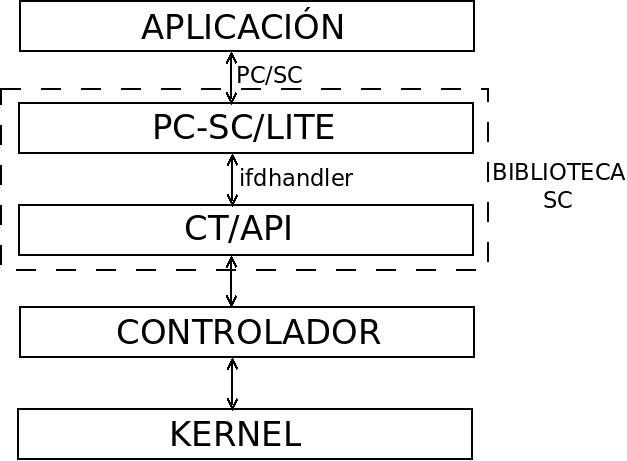
\includegraphics[scale=.4]{Imagenes/SW_sc1.jpg} 
  \end{center}
  \caption{Capas de software de trabajo}\label{Fig:capas} 
\end{figure}

En una primera etapa y para simplificar el desarrollo y la depuración del software, las capas empleadas fueron las que se muestran en la figura \ref{Fig:capas0}.


\begin{figure}[H]
\centering
  \begin{center}
  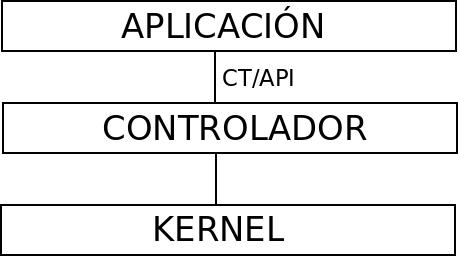
\includegraphics[scale=.4]{Imagenes/SW_sc2.jpg} 
  \end{center}
  \caption{Capas de software en una primera etapa}\label{Fig:capas0} 
\end{figure}

\bigskip
A continuación se describen las capas asociadas a la figura \ref{Fig:capas}.

\bigskip
\leftline{Controlador:}
El kernel es el encargado de manipular directamente los registros del puerto serial, las interrupciones que desde éste se generan y la ISR para atender las interrupciones.
La implementación del controlador del lector de tarjetas se basó en el controlador serial de Linux a través de su estructura “termios” \cite{termios}. Esta estructura permite configurar todos los parámetros necesarios para la comunicación serial como ser, baud rate, cantidad de bits por byte, bit de paridad, bit de parada entre otros. Las funciones read y write permiten la lectura y escritura de los bytes de datos que son recibidos y transmitidos por el puerto serial.

Dentro del proyecto MUSCLE/PCSCLite existe código ejemplo de controladores de lectores de tarjetas de contacto que son compatibles con la biblioteca, si bien el desarrollo se basó en alguno de ellos, como el hecho de usar el mismo nombre de funciones, su contenido fue desarrollado específicamente para controlar el hardware específico del prototipo RF$^{2}$.

\bigskip
\leftline{CT/API (Card Terminal / Application Programming Interface):}
Por encima del controlador serial se encuentra CT/API \cite{ctapi}, una interfaz definida por varias empresas (entre las que se incluye Telekom Alemania) en la década de los noventa, que permite encapsular el controlador específico de cada lector de tarjetas, de manera que la aplicación final no se vea afectada al cambiar un lector por otro.
Esta interfaz de programación está formada tan solo por 3 funciones, CT\_init, CT\_data y CT\_close, que permiten la inicialización del lector, la transferencia de datos entre host/lector o host/tarjeta (host se refiere a la SBC o PC donde se encuentra conectado el lector de tarjetas de contacto) directamente y el cierre de la comunicación.\\
CT\_init se encarga del pasaje de parámetros a la capa del controlador, para la configuración del puerto de comunicación entre el host y el lector de tarjetas. Los parámetros en uso aquí son: la tasa de transferencia de datos, el número de bits por cada byte, el tipo de paridad empleado y el puerto serie a ser utilizado.\\
CT\_data es la función encargada de transferir comandos y datos hacia y desde la tarjeta o hacia y desde el lector (en caso que el mismo esté formado por un ASIC o microprocesador). La manera de diferenciar desde donde es enviado el dato, es a través de un parámetro pasado a esta función, y de forma análoga se determina el destino del mensaje. El protocolo usado para la transferencia de datos es T=0, orientado a bytes y del cual pueden conocerse más detalles en \cite{SCHb}.\\
CT\_close es la contracara de  CT\_init, se encarga de cerrar la comunicación con el lector. Lo que hace básicamente es liberar el handle (puntero) asociado al puerto serial.\\

\bigskip
Las funciones de apertura y cierre de la comunicación no necesitan ser modificadas, son similares en todos 
los controladores de lectores seriales compatibles con la biblioteca. Por otro lado la función CT\_data debió ser sustancialmente modificada para lograr el intercambio de datos a partir del protocolo T=0.

\bigskip
Para el caso en que los comandos y/o datos estén dirigidos hacia el lector, existe otra especificación, llamada CT/BCS \cite{ctbcs} (Card Terminal / Basic Command Set), donde se encuentran definidos una serie de comandos básicos para el manejo del lector. Estos comandos se nombran a continuación y se da una breve descripción.

\bigskip
RESET CT permite reiniciar el lector o tarjeta (en el caso de ser un lector mudo); de manera opcional puede devolver el ATR.

REQUEST ICC tiene como objeto devolver el ATR de la tarjeta una vez que la misma se encuentra ubicada en el zócalo del lector.

GET STATUS es empleado para conocer información sobre el lector o si la tarjeta está insertada y eléctricamente conectada en el lector. 

EJECT ICC genera la desactivación eléctrica de la tarjeta.

\bigskip
\leftline{IFDHandler:}
El siguiente componente en este stack de capas es ifdhandler \cite{ifdhandler}, no es otra cosa que un conjunto de funciones formando una API, empleada por pcsclite para encapsular el manejo del hardware de  lectores cuyos fabricantes quieran cumplir con las especificaciones PC/SC \cite{pcsclite_esp}. Una ventaja importante de esta API es que le permite a pcsclite operar tanto con lectores de puerto serial como con lectores de puerto USB.
Esta capa de software podría usarse directamente sobre el controlador del lector, prescindiendo de CT/API, aunque se decidió mantenerla por motivos de simplicidad ya que sólo es necesario sustituir la capa de aplicación por las restantes capas superiores como se indica en las figuras anteriores.

\bigskip
Las funciones que contiene esta capa de software fueron modificadas para que contengan a su vez las funciones de CT/API, y de esta manera hacer más fácil de integrar el controlador del lector con la biblioteca PCSCLite.

\bigskip
En lo que sigue se enumeran algunas de las funciones de esta API y se describen brevemente. Por más detalles ver el manual ifdhandler \cite{ifdhandler}.

\bigskip
IFDHCreateChannel establece el canal de comunicación con el lector. Para conseguirlo usa un parámetro llamado Channel, que indica cual es el puerto serial a usar, por ejemplo para el caso de Linux /dev/ttySx (x es el número que corresponda).

IFDHCloseChannel implementa la acción opuesta a la función anterior, cerrando el canal de comunicación con el lector de tarjetas.

IFDHGetCapabilities permite obtener las capacidades específicas del lector o de la tarjeta insertada en el mismo.

IFDHPowerICC se encarga del control de las señales de alimentación y reset que el lector suministra a la tarjeta. Desempeña tres acciones posibles, encendido, reset y apagado de la tarjeta.

IFDHTransmitToICC se encarga de la transferencia de datos con la tarjeta a través de alguno de los protocolos disponibles, como ser T=0 o T=1.

IFDHICCPresence retorna el estado de la tarjeta insertada en el zócalo del lector.

\bigskip
\leftline{PCSCLite:}
Por arriba de ifdhandler se encuentra la biblioteca pcsclite, ésta contiente todas las funciones necesarias para establecer la comunicación con un lector y la tarjeta conectada a éste último. Para el uso del controlador encapsulado por ifdhandler desde pcsclite es necesario seguir los pasos de configuración detallados en el apéndice \ref{anx_pcsc_inst}.

\bigskip
\leftline{Aplicación final:}
Por arriba de todas las capas descritas antes, se encuentra la aplicación del prototipo que hace uso de las funciones suministradas por pcsclite y donde se encuentran definidos los comandos APDU específicos con los que opera la tarjeta de contacto. Por razones de seguridad no se nos permite difundir la lista de comandos que son usados para la comunicación con el módulo SAM.


\bigskip
\leftline{\bf{Software RFID}}
A continuación se detallan los cambios introducidos en la librfid para el correcto funcionamiento del lector/escritor RFID utilizando librfid-tool.

En la figura \ref{sw_RFID} se detalla la capa de software RFID.

\begin{figure}[H]
\centering
  \begin{center}
  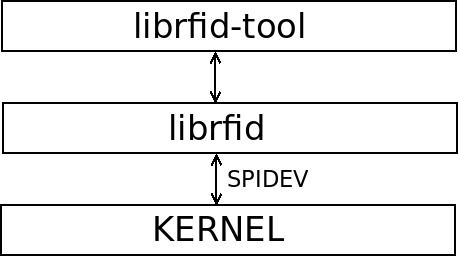
\includegraphics[scale=.4]{Imagenes/librfid-tool.jpg} 
  \end{center}
  \caption{Capa de software RFID}\label{sw_RFID} 
\end{figure}


\bigskip
Se analizó el código principal de la aplicación librfid-tool y se vio que dentro del directorio utils en el archivo common.c se encuentra la función reader\_init la cual busca un lector/escritor entre los soportados. Esta función no tenía implementada una búsqueda para dispositivos conectados por SPI. Por lo tanto se tuvieron que agregar las siguientes líneas a la función para que el funcionamiento fuera posible:

\begin{verbatim}
rh = rfid_reader_open("/dev/spidev3.0", RFID_READER_SPIDEV);
if (!rh) {
    fprintf(stderr, "No SPIDEV found\n");
    return -1;
}
\end{verbatim}

Este cambio permitió detectar la interfaz SPI (spidev3.0). Algo a tener en cuenta, es que como en Linux las interfaces están asociadas a un archivo, el hecho de abrir el archivo no implica que haya nada conectado en esa interfaz. Por esta razón, la búsqueda de un lector/escritor conectado por interfaz SPI se realiza en última instancia.

\bigskip
Otro cambio fundamental es en la frecuencia de reloj del puerto SPI. Se incrementa a 10MHz, ya que con la frecuencia establecida por defecto en la librfid (1MHz) el lector/escritor RFID no funciona correctamente. 

Toda la configuración de la comunicación por SPI se encuentra en rfid\_reader\_spidev.c que está en el directorio fuente src.

La función que se modificó es spidev\_open y el cambio se muestra a continuación:

\begin{verbatim}
tmp = 10e6; /* 10 MHz */
if (ioctl(spidev_fd, SPI_IOC_WR_MAX_SPEED_HZ, &tmp) < 0)
    goto out_rath;
\end{verbatim}

Se implementaron las funciones adecuadas  para el manejo del pin RST\_RF, el cual puede encender y apagar el lector/escritor RFID diseñado.

\bigskip
Después de estudiadas las funciones que provee la herramienta librfid-tool, se estudió la posibilidad de su uso para la aplicación RF$^{2}$. 

Aunque sus funciones  son muy útiles, la gran mayoría no sirven completamente para la aplicación RF$^{2}$ debido a que fueron definidas para otros propósitos. 

Es de interés, que la herramienta librfid-tool siga manteniendo sus funcionalidades y pueda convivir con la aplicación RF$^{2}$, por lo que no se modificó el contenido de ninguna función de la herramienta. En el caso que alguna función fuera mayormente utilizable, se procedió a crear una nueva con los cambios necesarios.

Se implementaron la mayoría de las funciones, logrando compatibilidad con la biblioteca librfid. Entre las funciones creadas están las asociadas con la tarjeta RFID: autenticación según el tipo de clave, búsqueda de tarjetas próximas al lector, lectura y escritura de bloques de memoria, obtención del UID, etc.

\subsection{Aplicación final}

Para el desarrollo de la aplicación RF$^{2}$ se decidió trabajar sobre los fuentes de la herramienta librfid-tool, ya que maneja varias funciones de utilidad y es de ayuda a la hora de compilar para el armado de una aplicación completa. Se mantuvieron todas las opciones de la herramienta ya que son muy útiles y pueden ayudar en un futuro para establecer orígenes de fallas. No se modificó ninguna función de la aplicación original y cuando fue necesaria alguna modificación, se procedió a implementar una nueva.

\bigskip
Antes de seguir fue necesario entender el funcionamiento de las reglas de compilación creadas para la aplicación librfid-tool sobre librfid. En el directorio raíz, se encuentran los siguientes archivos importantes para el desarrollo del sistema: autogen.sh, configure.in, configure, Makefile.am, Makefile.flags.am, Makefile.in, Makefile.

\bigskip
A continuación se describe a grandes rasgos la utilidad de cada uno de estos archivos:

\bigskip
configure.in es el archivo de configuración con el cual se crea el archivo configure.


Makefile.am es el archivo que establece las reglas de compilación (orden, dependencias, etc) y es con el cual se crea el archivo Makefile.in. Diferentes Makefile.am se encuentran en los subdirectorios de la librfid, por lo que se crea un Makefile.in dentro de cada subdirectorio.


Makefile.flags.am es un archivo con banderas establecidas para el sistema. Este archivo está incluido en todos los Makefile.am de la aplicación.


autogen.sh es un script que se encarga de crear los archivos configure y Makefile.in, cada uno de ellos creados a partir de los archivos correspondientes antes mencionados.

Al ejecutar el archivo configure, éste establece la configuración que necesita el Makefile.in para conocer las reglas de compilación que se van a usar y algunos parámetros extra. Luego de este proceso se generan los Makefile.

El archivo Makefile es el que conoce las reglas de compilación, las dependencias y las opciones elegidas para el desarrollo. Sabe incluso donde se encuentran los demás Makefile para ejecutarlos cuando sea necesario.

\bigskip
Cada subdirectorio tiene reglas locales de construcción de sus objetos y a su vez se ayudan mutuamente para lograr una aplicación más completa. Desde el Makefile principal se controla que todo funcione correctamente.
Para saber más sobre reglas de compilación puede visitarse \cite{Make}.

\bigskip
La aplicación RF$^{2}$ utiliza otras bibliotecas además de librfid, además estas bibliotecas van a interactuar entre sí, lo que lleva a que aparezcan nuevas dependencias. Por lo tanto, es necesario modificar las reglas de compilación.

\bigskip
Se agregó en el raíz de la librfid el directorio rf2 en el cual se encuentran subdirectorios con los fuentes necesarios para la comunicación con el display, leds, buzzer, tarjeta de contacto y otros utilitarios, formando la estructura que se muestra en la figura \ref{est_RF2}. 


\begin{figure}[H]
\centering
  \begin{center}
  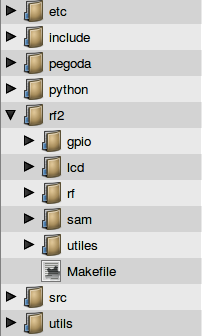
\includegraphics[scale=.5]{Imagenes/estructura_librfid.png} 
  \end{center}
  \caption{Estructura de árbol de aplicación RF$^{2}$}\label{est_RF2} 
\end{figure}

gpio incluye fuentes para el manejo de los GPIO.

lcd incluye fuentes para el manejo del display.

rf incluye fuentes con funciones extra de utilidad para el manejo del lector/escritor RFID diseñado.

sam incluye los fuentes para la comunicación con la tarjeta de contacto.

utiles incluye fuentes con funciones útiles de la aplicación.

\bigskip
Dentro de cada uno de estos directorios se encuentra un archivo Makefile con las reglas de compilación correspondientes a cada uno.

\bigskip
Las modificaciones a los archivos de construcción de la aplicación para que contemplen el agregado del directorio rf2, como la creación de nuevas reglas para la construcción dentro de éste, se detallan a continuación.

\bigskip
Antes que nada se decidió modificar los archivos Makefile.am para que sepan de la existencia del nuevo directorio. Se modifican estos archivos debido a que nunca son borrados. Por ejemplo, si los cambios se hacen sobre los Makefile.in, puede pasar que en algún momento se regeneren borrando los cambios que se hicieron. Además, luego de entender la estructura y funcionamiento de estos archivos, es más fácil incluir una modificación en Makefile.am que en un Makefile.in o Makefile directamente.

Dentro del directorio utiles, se creó el archivo Variables\_Make que establece el valor de algunas variables específicas de la aplicación RF$^{2}$ como ser CC\_arm que hace referencia al gcc asociado con la herramienta de croscompilación para ARM. 

\bigskip
Makefile.flags.am:
Aquí se indicó que se agregue rf2 a la ruta de búsqueda de archivos encabezados.

\begin{verbatim}
INCLUDES = \$(all_includes) -I$(top_srcdir)/include 
-I\$(top_srcdir)/rf2
\end{verbatim}

Makefile.am en el raíz:

\begin{verbatim}
include rf2/utiles/Variables_Make
\end{verbatim}
Con esto se aseguró que el resto de los subdirectorios pertenecientes a la librfid, sepan los valores de las variables específicas de la aplicación RF$^{2}$.

\bigskip
Luego se incluye el directorio rf2 a la aplicación, teniendo en cuenta que solo se va a incluir cuando se use un lector/escritor RFID con iterfaz SPI.
\begin{verbatim}
if ENABLE_SPIDEV 
SUBDIRS += rf2 
endif
\end{verbatim}

\bigskip
Makefile.am en utils:
Este es el cambio más dificil de entender y surge de la observación del Makefile.in generado cada vez (prueba y error). Como la aplicación RF$^{2}$ se basa en la modificación de los fuentes de la herramienta librfid-tool, se deben agregar todas las dependencias con archivos del nuevo subdirectorio rf2.

\begin{verbatim}
librfid_tool_SOURCES = librfid-tool.c librfid-tool.h 
common.c common.h ../rf2/gpio/gpio.c ../rf2/gpio/gpio.h 
../rf2/rf/rc632_utils.c ../rf2/rf/rc632_utils.h 
../rf2/lcd/lcd16x2.c ../rf2/lcd/lcd16x2.h ../rf2/sam/sam.c 
../rf2/sam/sam.h ../rf2/sam/sam_util.c ../rf2/sam/sam_util.h 
../rf2/utiles/utiles.c ../rf2/utiles/utiles.h
\end{verbatim}

Cada .h y .c se traduce en un .o al crear el Makefile.in.

\bigskip
Otro cambio necesario, ya que si no se incluye provoca errores de compilación, es el siguiente.

\begin{verbatim}
mifare_tool_SOURCES = mifare-tool.c common.c 
../rf2/gpio/gpio.c ../rf2/rf/rc632_utils.c 
../rf2/lcd/lcd16x2.c ../rf2/sam/sam.c 
../rf2/sam/sam_util.c ../rf2/utiles/utiles.c
\end{verbatim}

mifare-tool es otra herramienta de la librfid.

\bigskip
Luego se creó dentro del directorio rf2 un archivo Makefile que es el que ordena la construcción de todos los objetivos dentro de cada subdirectorio.

\begin{verbatim}
include utiles/Variables_Make 

all: gpio/gpio.o rf/rc632_utils.o lcd/lcd16x2.o 
sam/sam.o utiles/utiles.o 

gpio/gpio.o: 
	$(MAKE) -C gpio 

rf/rc632_utils.o: 
	$(MAKE) -C rf 

lcd/lcd16x2.o: 
	$(MAKE) -C lcd 

sam/sam.o: 
	$(MAKE) -C sam 
	 
utiles/utiles.o: 
	$(MAKE) -C utiles 

install: 

clean: 
	rm -f *.o 
	$(MAKE) -C gpio clean 
	$(MAKE) -C rf clean 
	$(MAKE) -C lcd clean 
	$(MAKE) -C sam clean 
	$(MAKE) -C utiles clean 

distclean: clean
\end{verbatim}

\bigskip
En este caso \$(MAKE) -C “directorio” indica que la regla de construcción del objetivo se encuentra en “directorio”.

\bigskip
Se implementó una función de inicialización, la cual inicializa todos los periféricos al arrancar la aplicación RF$^{2}$.

Se agregó una nueva opción (n) en el main de la aplicación librfid-tool que llama a la función principal(). Ésta es la función principal de la aplicación RF$^{2}$. De este modo no se modifica el main original de librfid-tool (solo se agrega la opción n) y se dejan las opciones por defecto.
Se hizo uso de algunas funciones ya escritas y se crearon otras. En este punto no se modificó ninguna función de la aplicación original y cuando fue necesaria alguna modificación, se procedió a implementar una nueva función con las modificaciones previstas.
Luego viene la etapa de croscompilación de la aplicación para ser probada en la SBC.

\bigskip
Croscompilación de la aplicación final:
Para guardar el resultado de la croscompilación se creó un directorio work en el home del usuario.

\bigskip
\centerline{\$ ./autogen.sh}
Este paso es necesario siempre que se modifiquen los Makefile.am, en otro caso no. Se recuerda que este script genera los archivos Makefile.in y configure.

\bigskip
\centerline{\$ ./configure $--$enable-spidev $--$host=arm-angstrom-linux-gnueabi $--$prefix=/home/proyecto/work}

\bigskip
Se configura el sistema para lectores/escritores RFID con interfaz SPI, se indica la arquitectura de la SBC para la cual se compila y se indica el directorio donde se instala la aplicación. Luego de hecho esto ya no es necesario volver a ejecutarlo ya que los Makefile quedan creados con esta configuración.

\centerline{\$ make clean \&\& make -j5 \&\& make install}
Se construye la aplicación.

\bigskip
En el directorio work se encuentran cuatro nuevos directorios creados:

\bigskip
bin: incluye los binarios construidos.

include: directorio con los .h necesarios para correr la aplicación.

lib: la biblioteca en sí.

share: nada de utilidad.

\bigskip
El paso siguiente es el de copiar estos directorios en el sistema de archivos de la SBC.

\bigskip
Copia de archivos a la SBC:

\bigskip
Para realizar la copia conviene comprimir el resultado de la croscompilación y luego enviarlo a la SBC.

\centerline{\$ tar -czf rf2.tar.gz bin include lib share}

\bigskip
Luego de enviar el archivo comprimido, es necesaria la copia de estos directorios en el sistema de archivos de la SBC.

\bigskip
Instalación en la SBC:

\centerline{\$ tar -xf rf2.tar.gz -C /usr}
Esto descomprime los directorios creados anteriormente, dentro del directorio /usr.

\bigskip
Se ejecuta la aplicación RF$^{2}$:

\centerline{\$ librfid-tool -n}

